\section{Formal Problem Definition}

Let $G = (V,E)$ be a graph (directed or undirected), where
$V$ is the set of nodes and $E$
is the set of edges.

Let $A$ be a set of agents that want to reach a point
 $t \in V$. Every agent $i \in A$, is located in a node of the
 graph. Let $pos(i)$ be the position of the agent $i$.
  Furthermore, a function over $i$ is defined for 
  determining the cost of the displacement of the agents 
 through the graph $\lambda_i : E \longrightarrow \mathbb{R}^{\geq 0}$.

For the sake of avoiding inconsistencies in the knowledge
shared between agents, it is considered, without any loss
 in the problem generality, that $V$ and $E$ are common to
  all the agents. Nonetheless, the definition of the cost function
  $\lambda_i$ can change with each agent, allowing the latter
  have a $\lambda_i$ that is adjusted to fit its restrictions.

Let $path(i)$ having $i \in A$, be the path that the 
agent $i$ is tacking to reach node $t$.

The degree of ambush towards the node $t$ is defined as:

\begin{equation}
\Phi(t) = \dfrac{|\{ i : path(j) = <pos(j),\ \ldots,\ i,\ t>, j \in A\}|}
{\min(|\{ <i,t> : <i,t> \in E \} |,|A|) }
\label{equation-1}
\end{equation}	  

That is, the proportion of nodes adjacent to $t$, 
from which an agent in $A$ is reaching the goal, 
regarding the maximum number of adjacent nodes to $t$.
Naturally, $\Phi$'s range is defined as $0 \leq \Phi(t) \leq 1$.

The main objective of the proposed variation is to maximise
$\Phi$'s value, having path diversity as a top priority, over getting
all agents to walk the obvious optimal route.

\begin{figure}[htp]
\centerline{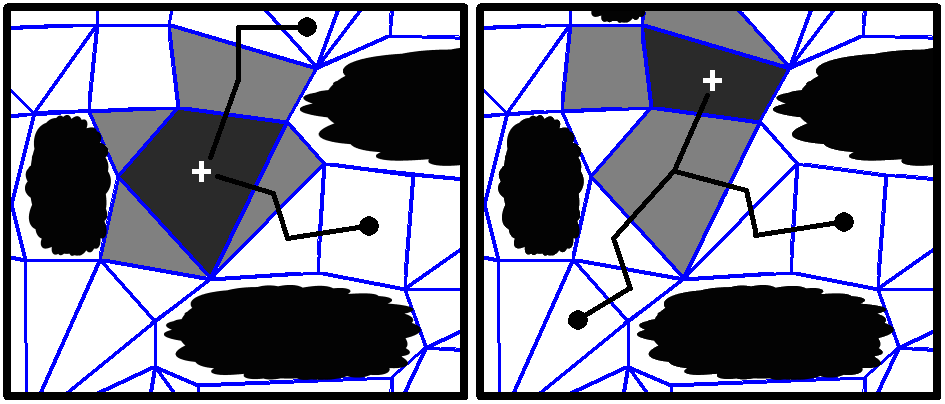
\includegraphics[width=0.6\columnwidth]{figures/ambush_rate.png}}
\caption{Ambush examples with values of $\Phi(t)$ 
	     1 y 0.5 respectively}
\label{fig:phi}
\end{figure}

See the example shown in figure \ref{fig:phi}. In the top image 
there are two agents situated where the black dots are. 
The objective that both agents want to reach is the white cross 
located in the dark gray polygon. The adjacent nodes to the goal 
are painted in light gray. Note that the number of polygons adjacent
to the objective is four. Out of those four, only two are being
considered in the agents paths. Therefore, the value of $\Phi(t)$
for this particular case is $\Phi(t) = \dfrac{2}{min(4,2)} = 1$.
It could seem that this ambush result is not optimal,
because there are two polygons that are left unreached.
 However, this is the greatest possible ambush degree, 
 given that only two agents are performing the strategy.

The image at the bottom shows an instance where, 
out of all the three polygons adjacent to the goal one, 
only one is being considered in the paths that the 
agents are tacking. For this case, the metric would
give the following result: $\Phi(t) = \dfrac{1}{min(3,2)} = 0.5$.

With the aim of not penalising cases like the first one, 
where the ambush was correctly performed, it is important
to consider the minimum between the number of agents and
the number of nodes adjacent to the objective node.